\hypertarget{index_preface_sec}{}\subsection{Preface\-: How to use this document}\label{index_preface_sec}
The documentation for Force\-Balance exists in two forms\-: a web page and a P\-D\-F manual. They contain equivalent content. The newest versions of the software and documentation, along with relevant literature, can be found on the \href{https://simtk.org/home/forcebalance/}{\tt Sim\-T\-K website}.

{\bfseries Users} of the program should read the {\itshape Introduction, Installation}, {\itshape Usage}, and {\itshape Tutorial} sections on the main page.

{\bfseries Developers and contributors} should read the Introduction chapter, including the {\itshape Program Layout} and {\itshape Creating Documentation} sections. The {\itshape \href{http://leeping.github.io/forcebalance/doc/html/api/roadmap.html}{\tt A\-P\-I documentation}}, which describes all of the modules, classes and functions in the program, is intended as a reference for contributors who are writing code.

Force\-Balance is a work in progress; using the program is nontrivial and many features are still being actively developed. Thus, users and developers are highly encouraged to contact me through the \href{https://simtk.org/home/forcebalance/}{\tt Sim\-T\-K website}, either by sending me email or posting to the public forum, in order to get things up and running.

Thanks!

Lee-\/\-Ping Wang\hypertarget{index_intro_sec}{}\subsection{Introduction}\label{index_intro_sec}
Welcome to Force\-Balance! \-:)

This is a {\itshape  theoretical and computational chemistry } program primarily developed by Lee-\/\-Ping Wang. The full list of people who made this project possible are given in the \hyperlink{index_credits}{Credits}.

The function of Force\-Balance is {\itshape automatic force field optimization}. Here I will provide some background, which for the sake of brevity and readability will lack precision and details. In the future, this documentation will include literature citations which will guide further reading.\hypertarget{index_background}{}\subsubsection{Background\-: Empirical Potentials}\label{index_background}
In theoretical and computational chemistry, there are many methods for computing the potential energy of a collection of atoms and molecules given their positions in space. For a system of {\itshape N} particles, the potential energy surface (or {\itshape potential} for short) is a function of the {\itshape 3\-N} variables that specify the atomic coordinates. The potential is the foundation for many types of atomistic simulations, including molecular dynamics and Monte Carlo, which are used to simulate all sorts of chemical and biochemical processes ranging from protein folding and enzyme catalysis to reactions between small molecules in interstellar clouds.

The true potential is given by the energy eigenvalue of the time-\/independent Schrodinger's equation, but since the exact solution is intractable for virtually all systems of interest, approximate methods are used. Some are {\itshape ab initio} methods ('from first principles') since they are derived directly from approximating Schrodinger's equation; examples include the independent electron approximation (Hartree-\/\-Fock) and perturbation theory (M\-P2). However, most methods contain some tunable constants or {\itshape empirical parameters} which are carefully chosen to make the method as accurate as possible. Three examples\-: the widely used B3\-L\-Y\-P approximation in density functional theory (D\-F\-T) contains three parameters, the semiempirical P\-M3 method has 10-\/20 parameters per chemical element, and classical force fields have hundreds to thousands of parameters. All such formulations require an accurate parameterization to properly describe reality.


\begin{DoxyImage}
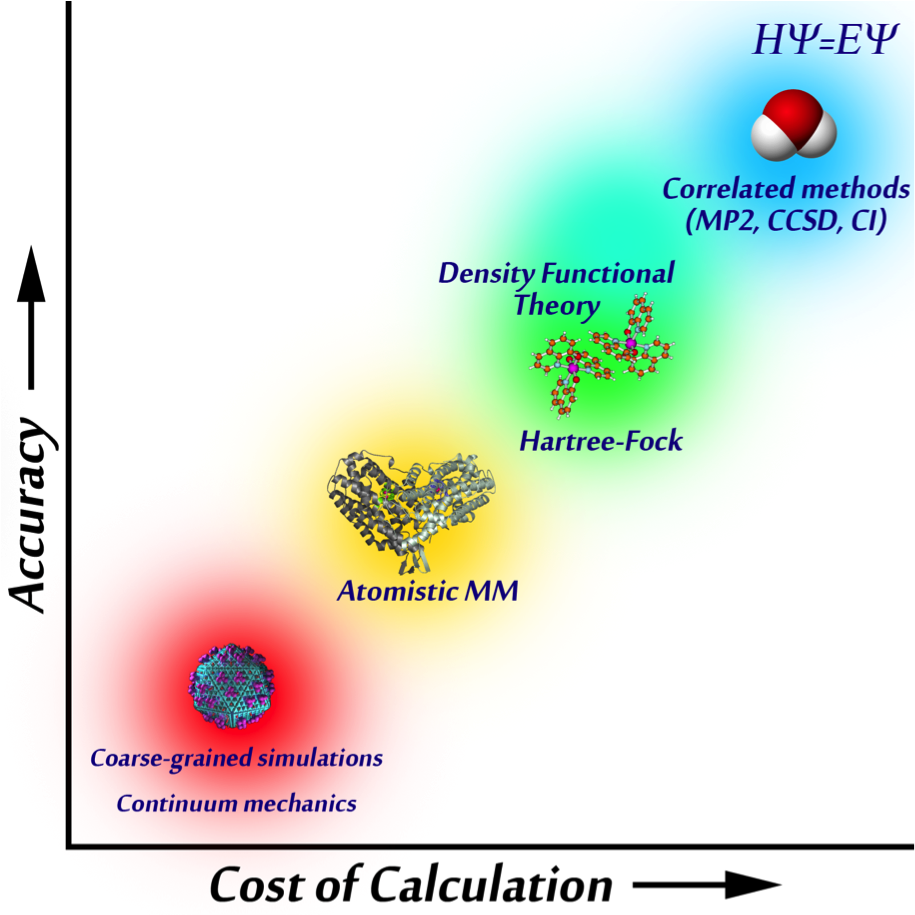
\includegraphics[width=10cm]{ladder.png}
\caption{An arrangement of simulation methods by accuracy vs. computational cost.}
\end{DoxyImage}


The main audience of Force\-Balance is the scientific community that uses and develops classical force fields. These force fields do not use the Schrodinger's equation as a starting point; instead, the potential is entirely specified using elementary mathematical functions. Thus, the rigorous physical foundation is sacrificed but the computational cost is reduced by a factor of millions, enabling atomic-\/resolution simulations of large biomolecules on long timescales and allowing the study of problems like protein folding.

In classical force fields, relatively few parameters may be determined directly from experiment -\/ for instance, a chemical bond may be described using a harmonic spring with the experimental bond length and vibrational frequency. More often there is no experimentally measurable counterpart to a parameter -\/ for example, electrostatic interactions are often described as Coulomb interactions between pairs of atomic point \char`\"{}partial charges\char`\"{}, but the fractional charge assigned to each atom has no rigorous experimental of theoretical definition. To complicate matters further, most molecular motions arise from a combination of interactions and are sensitive to many parameters at once -\/ for example, the dihedral interaction term is intended to govern torsional motion about a bond, but these motions are modulated by the flexibility of the nearby bond and angle interactions as well as the nonbonded interactions on either side.


\begin{DoxyImage}
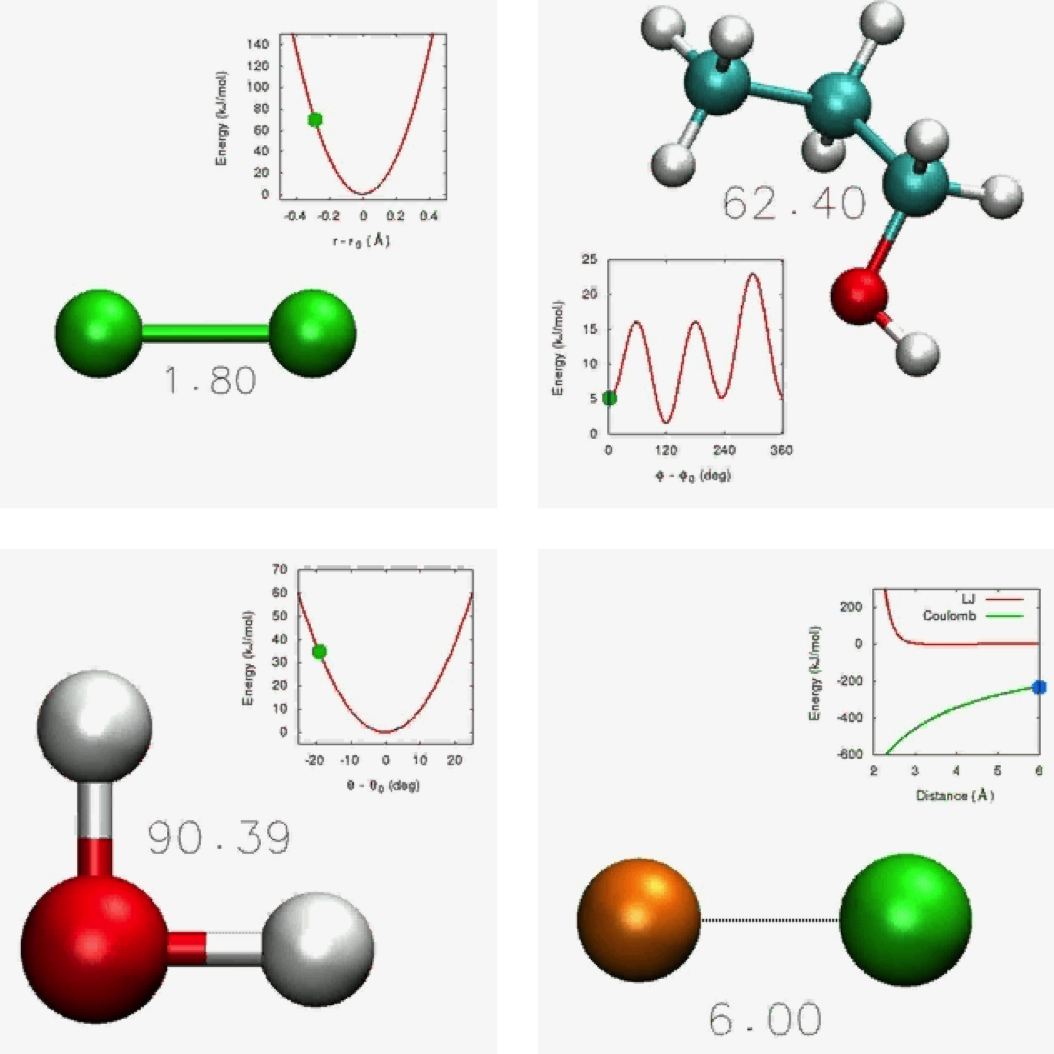
\includegraphics[width=10cm]{interactions.png}
\caption{An illustration of some interactions typically found in classical force fields.}
\end{DoxyImage}


For all of these reasons, force field parameterization is difficult. In the current practice, parameters are often determined by fitting to results from other calculations (for example, restrained electrostatic potential fitting (R\-E\-S\-P) for determining the partial charges) or chosen so that the simulation results match experimental measurements (for example, adjusting the partial charges on a solvent molecule to reproduce the bulk dielectric constant.) Published force fields have been modified by hand over decades to maximize their agreement with experimental observations (for example, adjusting some parameters in order to reproduce particular protein N\-M\-R structure) at the expense of reproducibility.\hypertarget{index_mission_statement}{}\subsubsection{Purpose and brief description of this program}\label{index_mission_statement}
Given this background, I can make the following statement. {\bfseries The purpose of Force\-Balance is to create force fields by applying a highly general and systematic process with explicitly specified input data and optimization methods, paving the way to higher accuracy and improved reproducibility. }

At a high level, Force\-Balance takes an empirical potential and a set of reference data as inputs, and tunes the parameters such that the simulations are able to reproduce the data as accurately as possible. Examples of reference data include energy and forces from high-\/level Q\-M calculations, experimentally known molecular properties (e.\-g. polarizabilities and multipole moments), and experimentally measured bulk properties (e.\-g. density and dielectric constant).

Force\-Balance presents the problem of potential optimization in a unified and easily extensible framework. Since there are many empirical potentials in theoretical chemistry and similarly many types of reference data, significant effort is taken to provide an infrastructure which allows a researcher to fit any type of potential to any type of reference data.

Conceptually, a set of reference data (usually a physical quantity of some kind), in combination with a method for computing the corresponding quantity with the force field, is called a {\bfseries target}. For example\-:


\begin{DoxyItemize}
\item A force field can predict the density of a liquid by running N\-P\-T molecular dynamics, and this computed value can be compared against the experimental density.
\end{DoxyItemize}


\begin{DoxyItemize}
\item A force field can be used to evaluate the energies and forces at several molecular geometries, and these can be compared against energies and forces from higher-\/level quantum chemistry calculations using these same geometries. This is known as {\bfseries force and energy matching}.
\end{DoxyItemize}


\begin{DoxyItemize}
\item A force field can predict the multipole moments and polarizabilities of a molecule isolated in vacuum, and these can be compared against experimental measurements.
\end{DoxyItemize}

Within a target, the accuracy of the force field can be optimized by tuning the parameters to minimize the difference between the computed and reference quantities. One or more targets can be combined to produce an aggregate {\bfseries objective function} whose domain is the {\bfseries parameter space}. This objective function, which typically depends on the parameters in a complex way, is minimized using nonlinear optimization algorithms. The result is a force field which minimizes the errors for all of the targets.


\begin{DoxyImage}
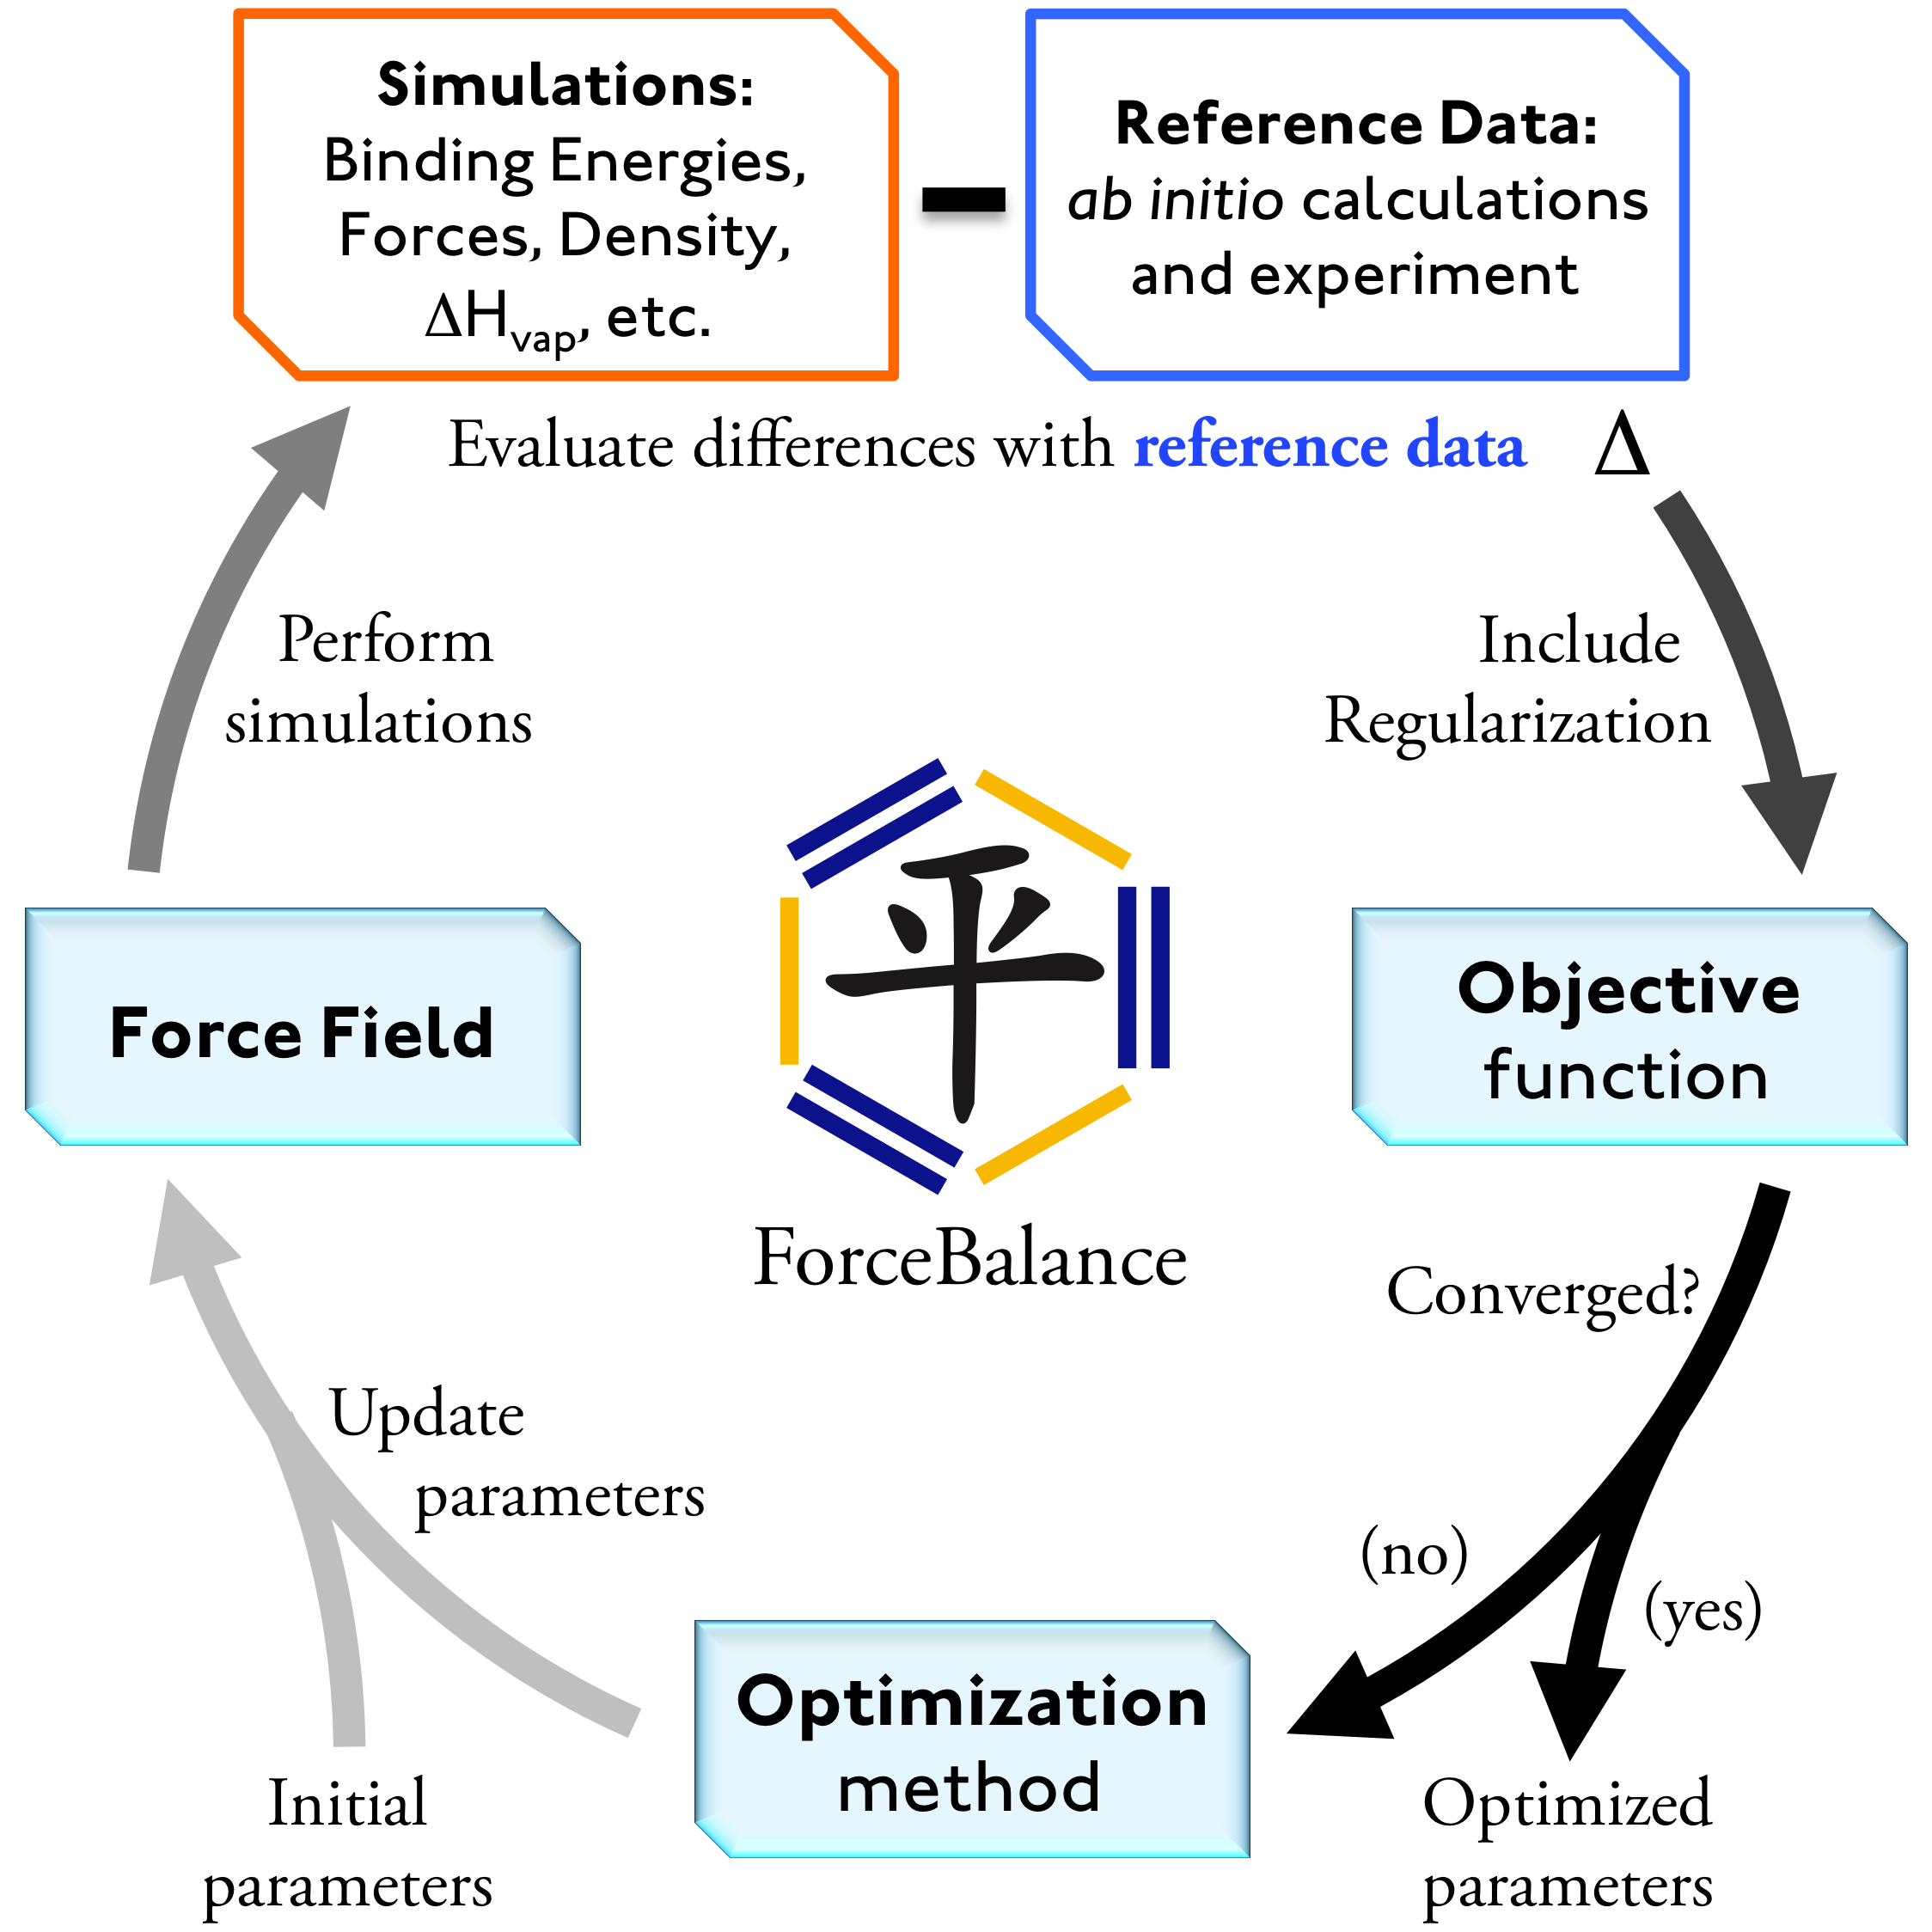
\includegraphics[height=10cm]{cycle.png}
\caption{The division of the potential optimization problem into three parts; the force field, targets and optimization algorithm.}
\end{DoxyImage}


The problem is now split into three main components; the force field, the targets, and the optimization algorithm. Force\-Balance uses this conceptual division to define three classes with minimal interdependence. Thus, if a researcher wishes to explore a new functional form, incorporate a new type of reference data or try a new optimization algorithm, he or she would only need to contribute to one branch of the program without having to restructure the entire code base.

The scientific problems and concepts that this program is based upon are further described in my Powerpoint presentations and publications, which can be found on the \href{https://simtk.org/home/forcebalance/}{\tt Sim\-T\-K website}.\hypertarget{index_credits}{}\subsection{Credits}\label{index_credits}

\begin{DoxyItemize}
\item Lee-\/\-Ping Wang is the principal developer and author.
\end{DoxyItemize}


\begin{DoxyItemize}
\item Troy Van Voorhis provided scientific guidance and many of the central ideas as well as financial support.
\end{DoxyItemize}


\begin{DoxyItemize}
\item Jiahao Chen contributed the call graph generator, the Q\-T\-P\-I\-E fluctuating-\/charge force field (which Lee-\/\-Ping implemented into G\-R\-O\-M\-A\-C\-S), the interface to the M\-O\-P\-A\-C semiempirical code, and many helpful discussions.
\end{DoxyItemize}


\begin{DoxyItemize}
\item Arthur Vigil contributed the unit testing framework and many unit tests, significant improvements to the automatic documentation generation, and various code improvements.
\end{DoxyItemize}


\begin{DoxyItemize}
\item Matt Welborn contributed the parallelization-\/over-\/snapshots functionality in the general force matching module.
\end{DoxyItemize}


\begin{DoxyItemize}
\item Vijay Pande provided scientific guidance and financial support, and through the Sim\-Bios program gave this software a home on the Web at the \href{https://simtk.org/home/forcebalance/}{\tt Sim\-T\-K website}.
\end{DoxyItemize}


\begin{DoxyItemize}
\item Todd Martinez provided scientific guidance and financial support. 
\end{DoxyItemize}